\chapter{Grundlegendes}
\label{Grundlegendes}
\section{Aufbau der Matrikelnummer}
\begin{figure}
	\centering
	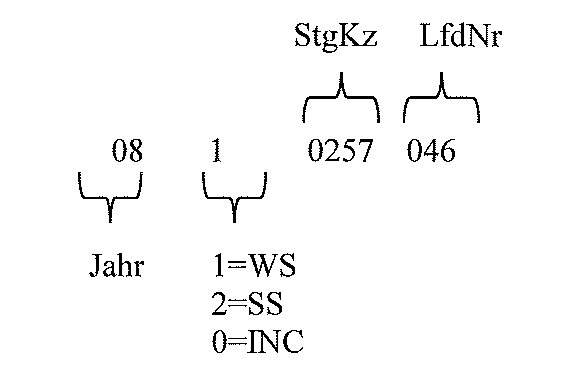
\includegraphics[width=0.75\textwidth]{Admin_AufbauMatrikelnummer.png}
	\caption{Aufbau der Matrikelnummer}
	\label{Aufbau der Matrikelnummer}
\end{figure}
Wenn an der dritten Stelle ein 2er steht (=SS) dann wird das Jahr um 1 verringert.

\section{Aufbau der UID}
\begin{figure}
	\centering
	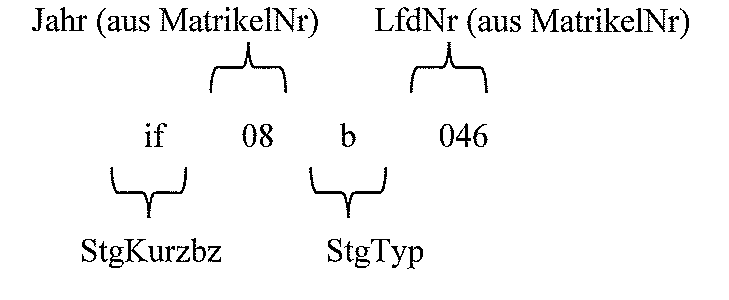
\includegraphics[width=0.75\textwidth]{Admin_AufbauUID.png}
	\caption{Aufbau der UID}
	\label{Aufbau der UID}
\end{figure}

\section{Variablen in public.tbl\_variable}
fas\_id - DEPRECATED\\
sleep\_time - DEPRECATED\\
\\
semester\_aktuell - Aktuell ausgew�hltes Studiensemester\\
kontofilterstg - wenn true dann werden nur die Buchungen des eigenen Studienganges angezeigt\\
emailadressentrennzeichen - Trennzeichen zwischen den Emailempf�ngern\\
\\
db\_stpl\_table - Studenplantabelle in die geschrieben wird (default: stundenplandev)\\
\\
ignore\_reservierung - Gibt an ob beim Verplanen im Stundenplan Reservierungen ignoriert werden sollen\\
ignore\_kollision - Gibt an ob beim Verplanen im Stundenplan Kollisionen ignoriert werden sollen\\
ignore\_zeitsperre - Gibt an ob beim Verplanen im Stundenplan Zeitsperren ignoriert werden sollen\\
